\documentclass[a4paper, 11pt]{article}

% Nécessaire
\usepackage[french]{babel}
\usepackage[utf8]{inputenc}
\usepackage[T1]{fontenc}
\usepackage{lmodern}
\usepackage{amsmath, amsthm}
\usepackage{amsfonts,amssymb}

% Marge
\usepackage{geometry}
\geometry{margin={2.2cm ,2cm}}

% Figures, graphiques
\usepackage{graphicx}
\usepackage{epsfig}
\usepackage{caption}

% Surlignage
\usepackage{alltt}

\usepackage[dvipsnames]{xcolor}
\usepackage{soul}
\usepackage{color}
\usepackage{colortbl}

% Indicatrice
\usepackage{dsfont}

\usepackage{multirow}
\usepackage{eurosym}
\usepackage{extarrows}

% Graphique
\usepackage{tikz}


% Titre
\title{Calibration et analyse de sensibilité du modèle}
\author{}
\date{}



\begin{document}
\maketitle

Le modèle possède cinq paramètres inconnus à calibrer, à savoir :
\begin{itemize}
 \item $\gamma$ le paramètre relatifs aux individus exogènes ;
 \item $p_m$ le paramètre régulant les échanges intra-bloc ;
 \item $\mu_{\text{ER}}$ la probabilité de survie à l'enherbement ras ;
 \item $\mu_{\text{EH}}$ la probabilité de survie à l'enherbement haut ;
 \item $k$ le paramètre lié à la capacité d'accueil des inflorescences.
\end{itemize}

\section{Qualité d'ajustement}

Avant une quelconque estimation des paramètres, nous avons besoin de mesurer la qualité de nos estimations. Pour ce faire, on utilisera une fonction pour comparer le nombre de larves estimées avec le nombre de larves observés. Pour définir cette fonction, on pose :
\begin{itemize}
 \item $m$, le nombre de jours entre la première observation et la dernière ;
 \item $n$, le nombre de relevés effectif;
 \item $t$, le nombre de jours passés depuis la première observation ;
 \item $t^j$, le nombre de jours entre la première observation et le $j^{\text{ème}}$ relevé.
\end{itemize}
(On a donc $t^1 = 0$ et $t^n = m$.)

La fonction est alors définie par
$$
f(y, \hat y) = \frac{\sqrt{\frac{1}{n}\sum_{j=2}^n\left( y^*_j - \hat y^*_j \right)^2}}{\max(y) - \min(y)},
$$
où 
$$y^*_j =  y_{t^j} \qquad \text{ et } \qquad \hat y^*_j = \frac{1}{t^j - t^{j-1}}\sum_{k=t^{j-1}}^{t^j} \hat y_k.$$
La figure~\ref{fig:calib} illustre le fonctionnement de la fonction. Appliquer la fonction à $n-1$ valeurs (correspondant aux relevés) plutôt qu'à chacun des $m$ jours (correspondant à l'étendue des relevés) est motivé par le fait que les relevés ne furent pas fait à des intervalles de temps régulier. Ce faisant, on évite d'attribuer plus d'importance aux relevés qui ont eu un écart relativement important avec le relevé précédent.

\begin{figure}[ht]
\centering
\begin{tikzpicture}[scale = 0.75]
 \draw [very thin, lightgray, opacity = 0.5] (0,0) grid (13.9, 8.4);
 \draw [->] (0, 0) -- (0, 8.5);
 \draw [->] (0, 0) -- (14, 0);
 \draw (1, 2) node{\textcolor{blue}{$\bullet$}};
 \draw (2, 2) node{\textcolor{blue}{$\bullet$}};
 \draw (3, 2) node{\textcolor{blue}{$\bullet$}};
 \draw (4, 2) node{\textcolor{blue}{$\bullet$}};
 \draw (5, 2) node{\textcolor{blue}{$\bullet$}};
 \draw (6, 2) node{\textcolor{blue}{$\bullet$}};
 \draw (7, 6) node{\textcolor{blue}{$\bullet$}};
 \draw (8, 6) node{\textcolor{blue}{$\bullet$}};
 \draw (9 , 5) node{\textcolor{blue}{$\bullet$}};
 \draw (10, 5) node{\textcolor{blue}{$\bullet$}};
 \draw (11, 5) node{\textcolor{blue}{$\bullet$}};
 \draw (12, 5) node{\textcolor{blue}{$\bullet$}};
 \draw (1, 2.1) node{\textcolor{red}{$\bullet$}};
 \draw (2, 2.9) node{\textcolor{red}{$\bullet$}};
 \draw (3, 3.6) node{\textcolor{red}{$\bullet$}};
 \draw (4, 4.2) node{\textcolor{red}{$\bullet$}};
 \draw (5, 4.6) node{\textcolor{red}{$\bullet$}};
 \draw (6, 4.9) node{\textcolor{red}{$\bullet$}};
 \draw (7, 4.9) node{\textcolor{red}{$\bullet$}};
 \draw (8, 4.7) node{\textcolor{red}{$\bullet$}};
 \draw (9, 4.3) node{\textcolor{red}{$\bullet$}};
 \draw (10, 3.6) node{\textcolor{red}{$\bullet$}};
 \draw (11, 3) node{\textcolor{red}{$\bullet$}};
 \draw (12, 2.2) node{\textcolor{red}{$\bullet$}};
 \draw [dashed] (0.8, 3.716) -- (6.2, 3.716) ;
 \draw [dashed] (6.8, 4.8) -- (8.2, 4.8) ;
 \draw [dashed] (8.8, 3.275) -- (12.2, 3.275) ;
 \draw (0.8, 3.616) -- (0.8, 3.816);
 \draw (6.2, 3.616) -- (6.2, 3.816);
 \draw (6.8, 4.7) -- (6.8, 4.9);
 \draw (8.2, 4.7) -- (8.2, 4.9);
 \draw (8.8, 3.175) -- (8.8, 3.375);
 \draw (12.2, 3.175) -- (12.2, 3.375);
 \draw (3.5, 3.716) node{\textcolor{red}{$\times$}};
 \draw (7.5, 4.8) node{\textcolor{red}{$\times$}}; 
 \draw (10.5, 3.275) node{\textcolor{red}{$\times$}};
 \draw (3.5, 2) node{\textcolor{blue}{$\times$}};
 \draw (7.5, 6) node{\textcolor{blue}{$\times$}}; 
 \draw (10.5, 5) node{\textcolor{blue}{$\times$}}; 
 \draw [<->] (3.5, 2.2) -- (3.5, 3.6);                  
 \draw [<->] (7.5, 5.8) -- (7.5, 5);
 \draw [<->] (10.5, 4.8) -- (10.5, 3.5);
 \draw [fill=white,white] (10.3, 7.01) rectangle (13.9, 8.4);
 \draw (12.2, 8) node {{\small Observation}};
 \draw (12.08, 7.5) node {{\small Estimation}};
 \draw (10.7, 8) node{\textcolor{blue}{$\bullet$}};
 \draw (10.7, 7.5) node{\textcolor{red}{$\bullet$}};
 \draw (6, 0.135) node[rotate = 180] {\textcolor{ForestGreen}{$\intercal$}};
 \draw (8, 0.135) node[rotate = 180] {\textcolor{ForestGreen}{$\intercal$}};
 \draw (12, 0.135) node[rotate = 180] {\textcolor{ForestGreen}{$\intercal$}};
\end{tikzpicture}
\caption{Schéma illustrant le fonctionnement de la fonction objectif. À chaque relevé effectif (marqueurs verts), on fait correspondre la période correspondant à ce relevé (segments en pointillés).
Et pour chacune de ces périodes, on calcule la moyenne des valeurs estimées (les croix rouges). On compare ensuite les moyennes ainsi calculées avec les valeurs observées associées (les croix bleues).}
\label{fig:calib}
\end{figure}


Par la suite, l'objectif sera de minimiser cette fonction.


\section{Analyse de sensibilité}

Afin d'avoir une meilleure idée  de l'influence des paramètres sur le modèle, on réalise une analyse de sensibilité du modèle. On utilisera la méthode Sobol, l'implémentation utilisée est décrite dans~\cite{sa}. Il n'y a cependant pas de méthode permettant d'avoir une idée des intervalles dans lesquels évoluent les paramètres. 
Si pour les probabilités il paraît normal de les faire évoluer entre 0 et 1, les intervalles pour les paramètres $\gamma$ et $k$ sont plus délicats à choisir.

On choisira ici l'intervalle $[0;0.1]$ pour $\gamma$ et l'intervalle $[1; 70]$ pour $k$. Ces choix sont motivés par des résultats de calibration antérieurs qui proposaient des valeurs pour lesdits paramètres dans des intervalles strictement inclus dans ceux qui seront utilisés. Cela reflètera ainsi au mieux le comportement réel du modèle.

Les résultats sont visibles sur la figure~\ref{fig:sa}. Il est intéressant de noter que les paramètres ont des effets différents d'un sous-bloc à l'autre, ce qui est rassurant. Le paramètre $\gamma$ est important pour les trois sous-blocs, avec des intéractions non-négligeables. Les probabilités de survie à la modalité de couverture du sol sont également important, variant selon les sous-blocs. Ainsi $\mu_{\text{ER}}$ apporte beaucoup de variance pour les sous-blocs «ER» et «PS»; il n'apporte aucune variance pour le sous-bloc «EH». Le paramètre $\mu_{\text{EH}}$ est important pour le sous-bloc «EH» et négligeable pour les deux autres. Le paramètre $p_m$ apporte une variance comparable pour les trois sous-blocs. Enfin, le paramètre $k$ n'a --- semble-t-il --- aucun impact sur le moodèle.


\begin{figure}[ht]
 \centering
 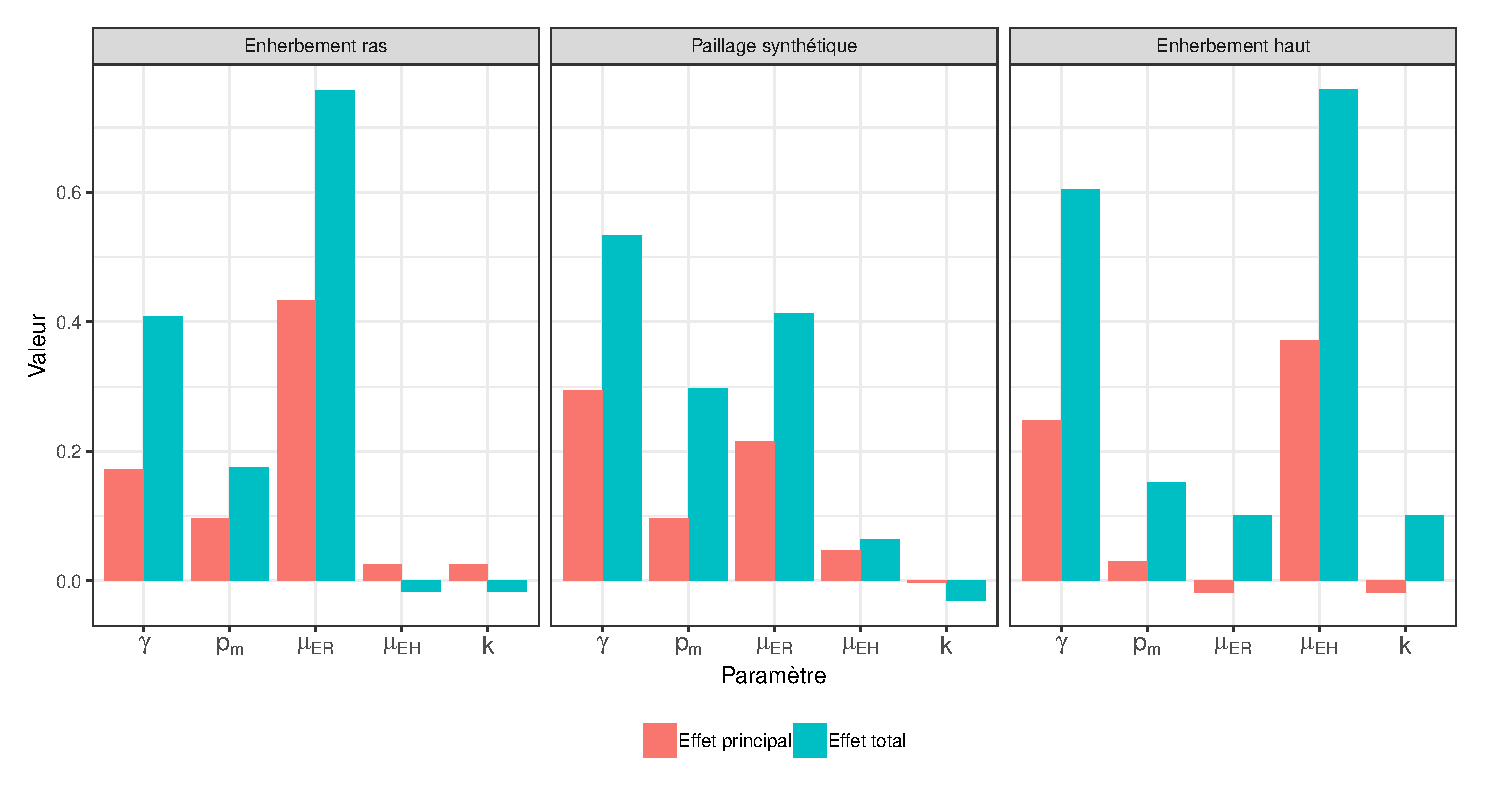
\epsfig{file = plots/sensitivity_analysis.eps, scale = 0.6}
 \caption{Analyse de sensitivité du modèle. Méthode Sobol}
 \label{fig:sa}
\end{figure}


\section{Calibration}

Une première calibration du modèle avec NSGA-II en prenant pour critère la qualité d'estimation sur chacun des trois sous blocs donne des résultats peu convenables. En effet, le paramètre $\mu_{\text{EH}}$ est presque toujours fixé à 0 (ou très proche). Cela peut s'expliquer pour deux raisons. Premièrement, ce paramètre n'est important que dans un seul des trois sous-blocs; il n'est donc pas très important pour le modèle dans sa globalité. Deuxièmement, le modèle (dans sa version actuelle) n'a que le paramètre $\gamma$ pour parvenir à une baisse en fin de saison. Il utilise donc en premier lieu le $\gamma$ puis complète au besoin avec des individus émergents (qui eux se multiplient sans moyen de stopper la dynamique).

Pour pallier ce problème, l'idée est d'alors de rajouter un critère permettant la préférence des individus émergents sur les individus exogènes. Mais pour cela, il faut d'abord enlever un des trois critères déjà présent car NSGA-II devient mauvais au delà de trois critères \cite{nsga3}.


À cette fin, on a lancé 5 répétitions de NSGA-II (\emph{popsize} = 100 et \emph{generations} = 200). On a ainsi pu récupérer 500 solutions accompagnés de la valeur de la \textit{NRMSE} produite sur chaque sous-bloc. Les corrélations trouvés sur ces valeurs sont les suivantes :
$$
\rho\left( ER, PS \right) = -0.869 \qquad \rho\left( ER, EH \right) = 0.761 \qquad \rho\left(PS, EH \right) = -0.943
$$
Les sous-blocs PS et EH sont très corrélés négativement. Baisser l'erreur de l'un entraîne une augmentation de l'autre. Comme le montre la figure~\ref{fig:cost} l'erreur associée à EH est plus grande que celle associée à PS. En retirant le critère PS, cela contribuera à baisser l'erreur sur l'enherbement haut de sorte que les erreurs entre PS et EH seront plus équilibrées. Cela libère également un critère permettant d'introduire notre nouveau critère.

\begin{figure}[ht]
 \centering
 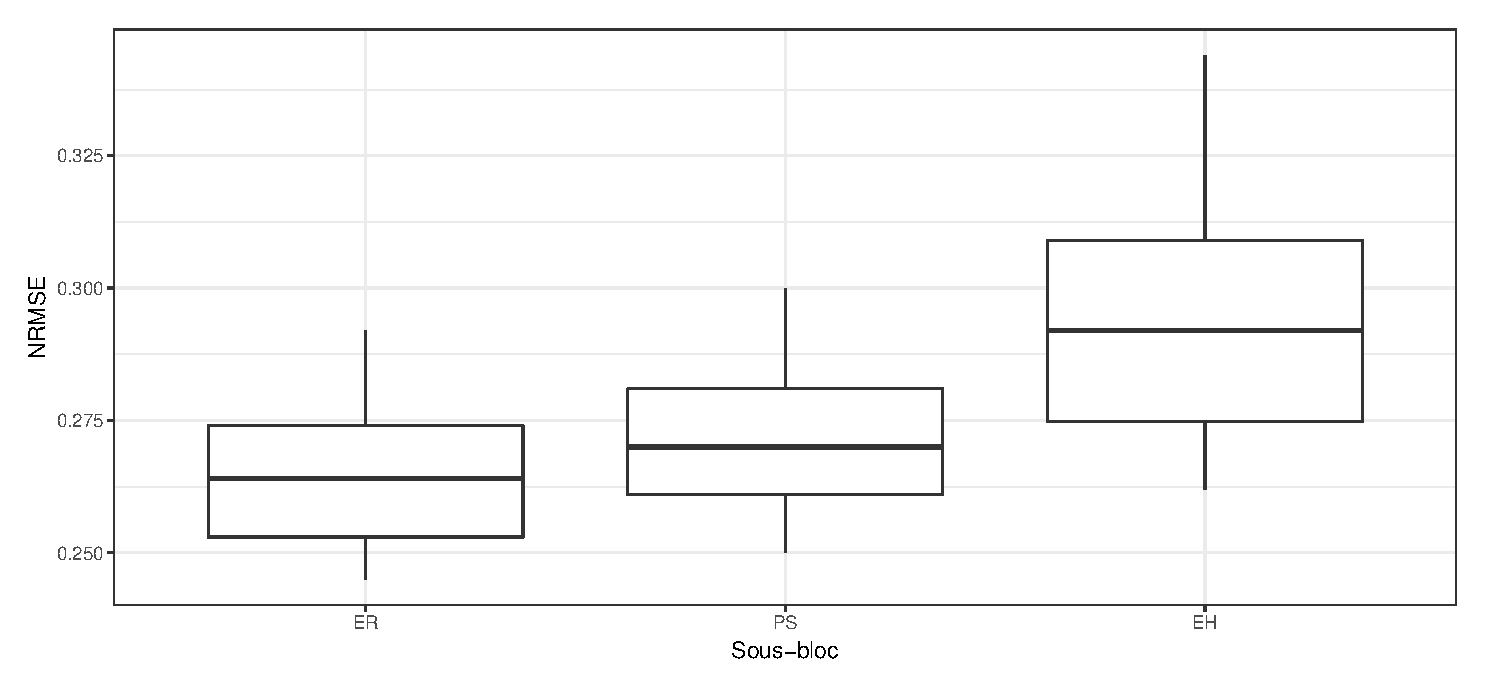
\epsfig{file = plots/comp_cost.eps, scale = 0.6}
 \caption{Comparaison des valeurs de la NRMSE des solutions proposées par NSGA-II en fonction des trois sous-blocs.}
 \label{fig:cost}
\end{figure}



Ce nouveau critère portant sur la préférence des émergents est défini par 
$$
\max \sum_{t, i}\frac{N_{t,i} - N_{t, i}^{\text{exo}}}{N_{t, i}}.
$$
Nos trois critères sont donc maintenant : ER, EH et la maximisation des émergents.



Il ne reste plus maintenant qu'à lancer NSGA-II plusieurs fois et à en extraire le front de Pareto.

\section{Résultats}

Pour la calibration des paramètres en fonction de nos trois critères, on relance NSGA-II 15 fois avec une taille de population de 300. Il s'avère que parmi les 4500 solutions certaines sont dominées par d'autres. Au final, il nous reste 1622 solutions.

Choisir la solution qui minimise la distance à 0 n'est pas toujours la solution la plus pertinente vis à vis de notre problème. Il peut être intéressant de rechercher, d'explorer parmi les solutions proposées. 

À cette fin, effectuer une ACP peut s'avérer intéressant\footnote{Une régression PLS2 serait même mieux dans la mesure où cela permettrait de mieux mettre en évidence l'impact des paramètres sur l'optimisation des critères.}. Ce fût chose faite, avec les valeurs de la \textit{NRMSE} pour chaun des trois sous-blocs et le critère de maximisation des émergents en variables actives et les cinq paramètres en variables supplémentaires. Les trois premiers axes capturent près de 99\% de l'inertie, on les sélectionne pour l'analyse. 
Les représentations des individus et des variables sur le plan $(1,2)$ sont visibles sur la figure~\ref{fig:pca}. 

\begin{figure}[ht]
 \centering
 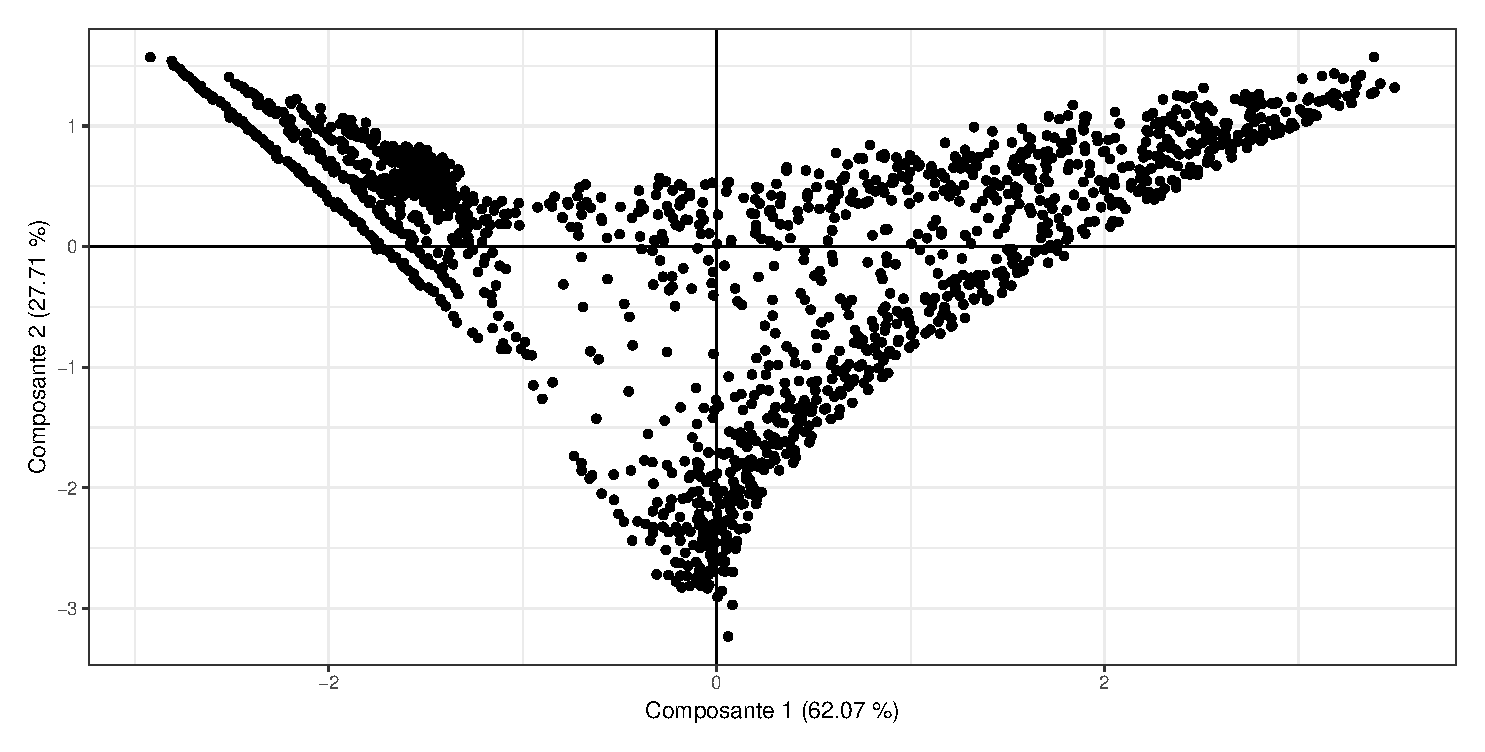
\epsfig{file = plots/pca12ind.eps, scale = 0.65}
 
 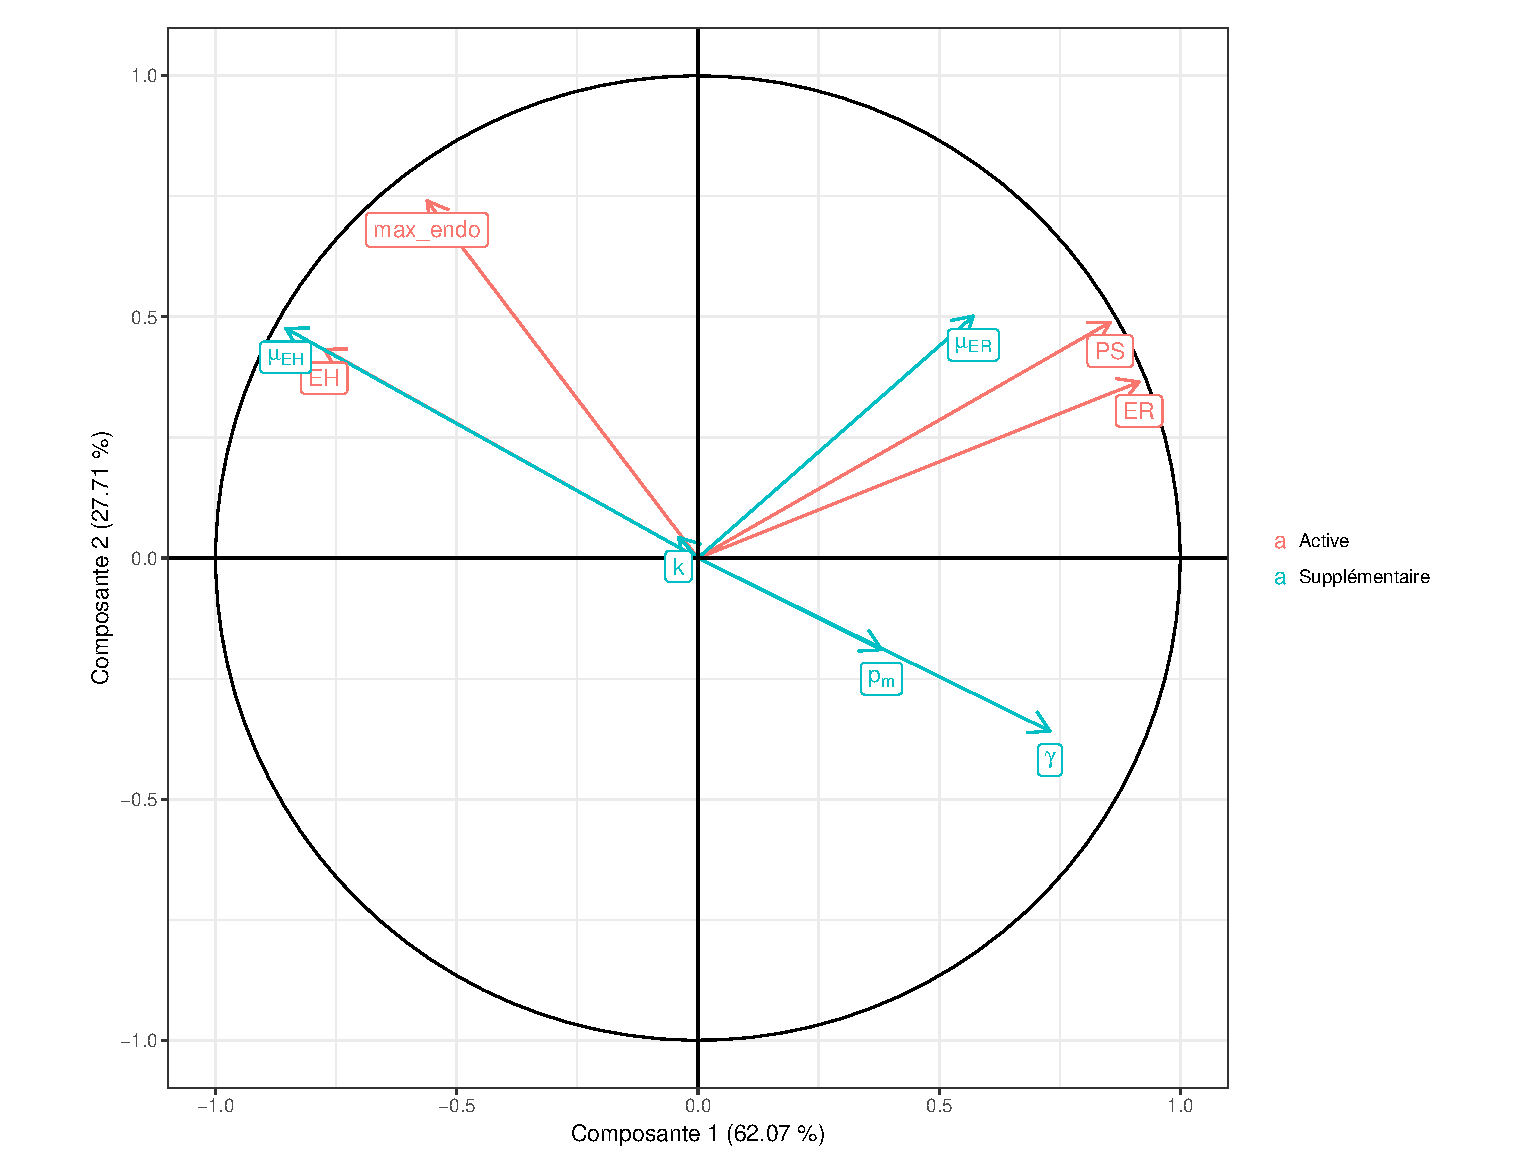
\epsfig{file = plots/pca12var.eps, scale = 0.50}
 
 \caption{Repésentation des individus (en haut) et des variables (en bas) sur le plan (1,2) qui capture 90\% de l'inertie.}
 
 \label{fig:pca}
\end{figure}

On observe la corrélation négative entre le critère de maximisation des émergents et le paramètre $\gamma$, ce qui est parfaitement logique : moins il y a d'individus exogènes, plus le modèle utlise les individus émergents pour ajuster aux données.
On observe aussi une très forte corrélation positive entre le critère EH et le paramètre $\mu_{\text{EH}}$. Cela signifie qu'une augmentation de $\mu_{\text{EH}}$ s'accompagne d'une augmentation du critère EH que l'on souhaite minimiser. Ce qui explique le fait que $\mu_{\text{EH}}$ était souvent fixé à 0 avant l'introduction du critère sur la maximisation des endogènes.
Un phénomène comparable --- mais de moindre envergure --- est visible pour $\mu_{\text{ER}}$ et le critère ER.

On observe une corrélation positive entre les critères ER et PS. Il y a aussi une corrélation positive entre les deux autre critères, mais il faut maximiser le critère de préférence des émergents et minimiser le critère EH : il y a donc un antagonisme entre l'amélioration de ces deux critères.



\begin{figure}[ht]
 \centering
 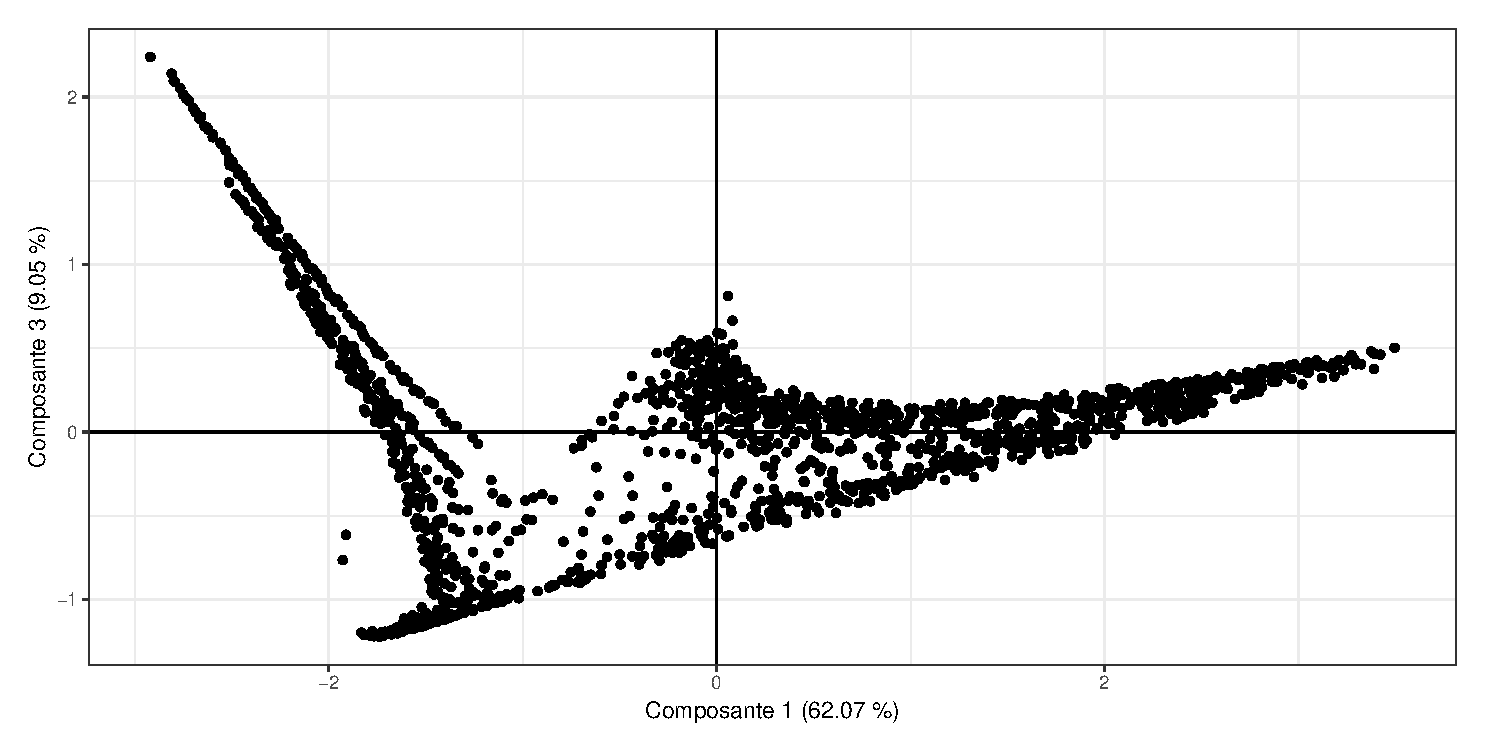
\epsfig{file = plots/pca13ind.eps, scale = 0.65}
 
 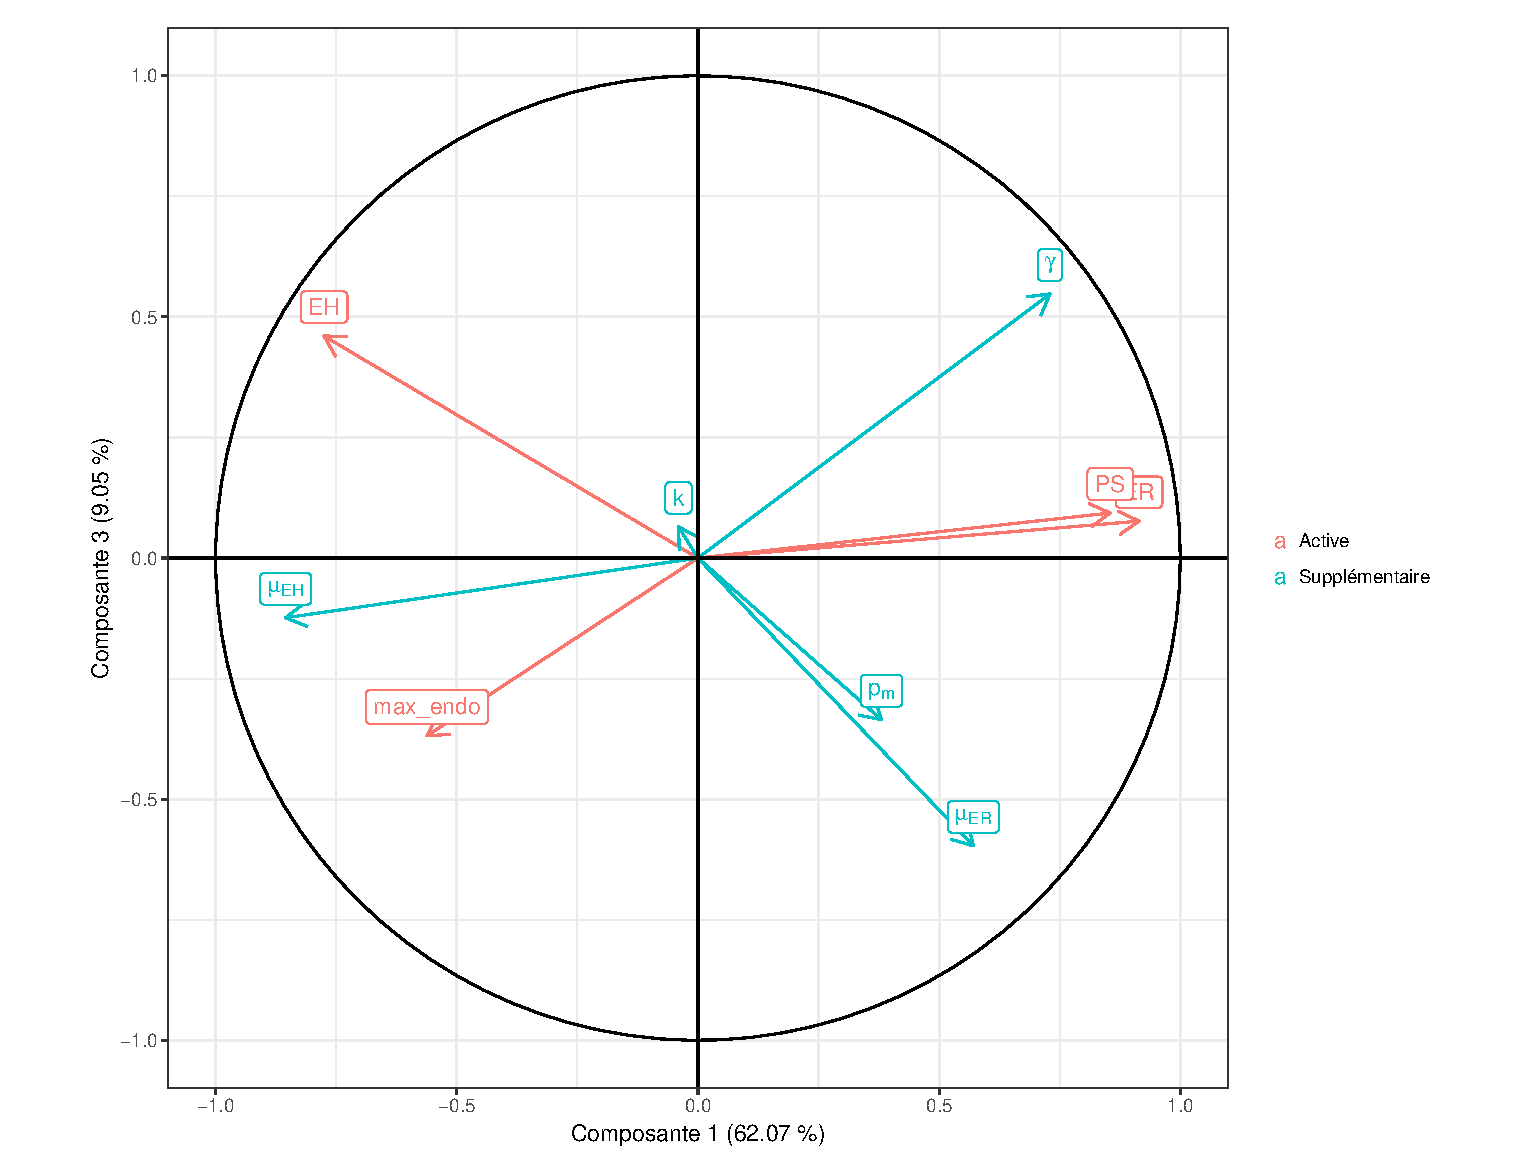
\epsfig{file = plots/pca13var.eps, scale = 0.50}
 
 \caption{Repésentation des individus (en haut) et des variables (en bas) sur le plan (1,3) qui capture 71\% de l'inertie.}
 
 \label{fig:pca2}
\end{figure}

Le plan $(1, 3)$ (figure~\ref{fig:pca2}) met en exergue des phénomènes moins évident. Il semblerait que le paramètre $\mu_{\text{EH}}$ soit corrélé négativement avec les critères PS et ER. Il en va de même pour le paramètre $\mu_{\text{ER}}$ et le critère EH. Ainsi, donc maximiser les paramètres $\mu_{\text{ER}}$ et $\mu_{\text{EH}}$ pourrait avoir de bonnes conséquences sur l'estimation dans certains sous-blocs.


En résumé, le plan $(1,2)$ --- qui capture 90\% de l'inertie --- montre que :
\begin{itemize}
 \item lorsque $\gamma$ est élevé, le critère de préférence des émergents n'est pas très bien respecté et le critère EH est bien respecté;
 \item lorsque $\mu_{\text{EH}}$ est élevé, le critère EH n'est pas bien respecté et le critère de maximisation des émergents est bien respecté;
 \item lorsque $\mu_{\text{ER}}$ est élevé, les critères ER et PS ne sont pas très bien respectés.
\end{itemize}
Le plan $(1, 3)$ --- qui capture 71\% de l'inertie --- montre que :
\begin{itemize}
 \item lorsque $\mu_{\text{EH}}$ est élevé, les critères ER et PS sont bien respectés;
 \item lorsque $\mu_{\text{ER}}$ est élevé, le critère EH est bien respecté.
\end{itemize}

En conclusion, les critères EH et préférence des émergents sont incompatibles. Ensuite, il n'y a pas de paramètres qui ait une valeur qui soit bénéfique pour tous les aspects du modèle. Ainsi, il va donc falloir trouver un compromis qui permette de n'être pas trop mauvais sur tous les critères.

\section{Exemples de solutions}

Pour être bon sur le critère de préférence des émergents, on peut sélectionner une solution ayant un $\gamma$ relativement faible (voir figure~\ref{fig:emer}). 

\begin{center}
\begin{tabular}{lllll}
$\gamma$ & $p_m$ & $\mu_{\text{ER}}$ & $\mu_{\text{EH}}$ & $k$\\
0.013 & 0.813 & 0.999 & 0.995 & 47.306
\end{tabular}
\end{center}


\begin{figure}[ht]
 \centering
 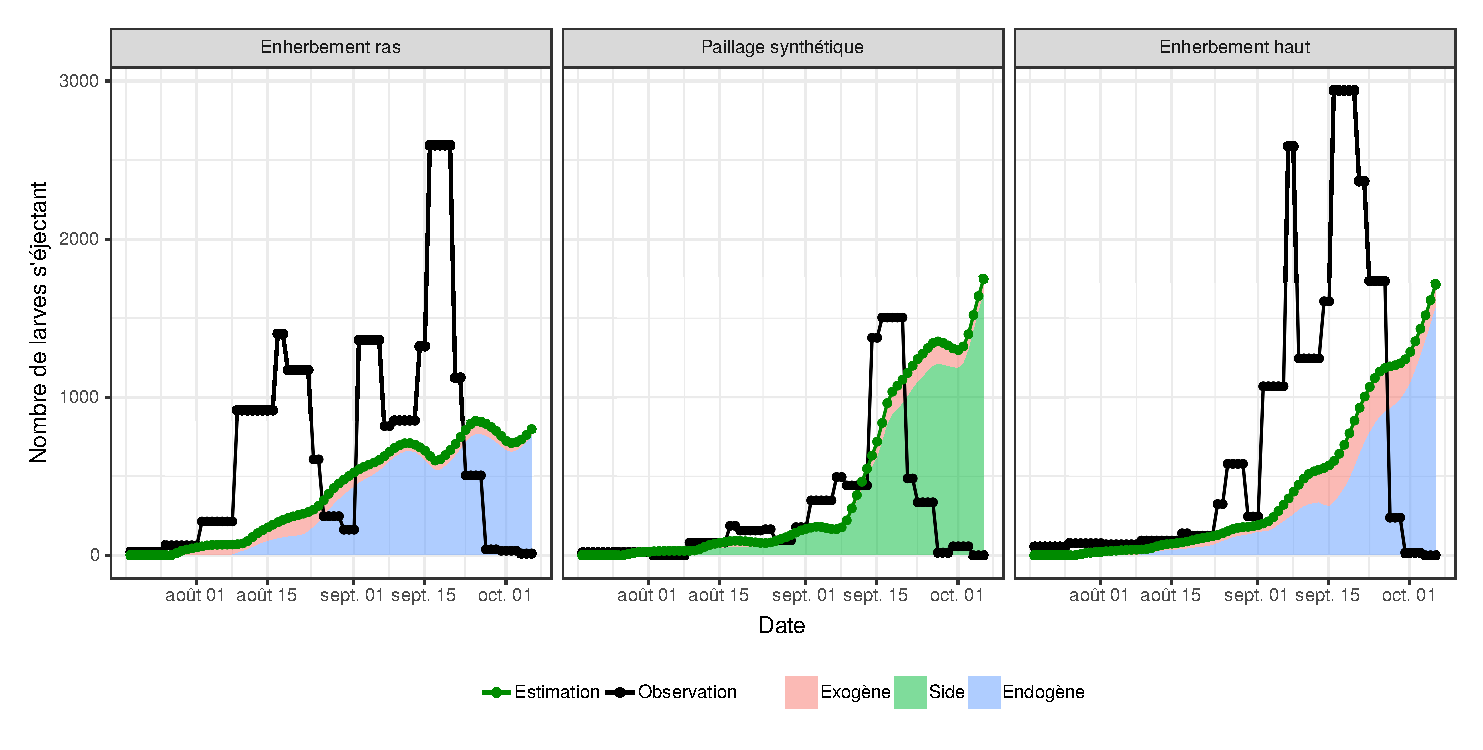
\epsfig{file = plots/max_emer.eps, scale = 0.65}
  
 \caption{Dynamiques estimées avec un jeu de paramètres vérifiant $\gamma < q_{0.1}\left( \gamma \right)$.}
 
 \label{fig:emer}
\end{figure}

Pour être bon sur les critères ER et PS, on peut sélectionner une solution ayant un $\mu_{\text{ER}}$ faible et un $\mu_{\text{EH}}$ élevé (voir figure~\ref{fig:erps}). 

\begin{center}
\begin{tabular}{lllll}
$\gamma$ & $p_m$ & $\mu_{\text{ER}}$ & $\mu_{\text{EH}}$ & $k$\\
0.046 & 0.790 & 0.497 & 0.971 & 12.543
\end{tabular}
\end{center}


\begin{figure}[ht]
 \centering
 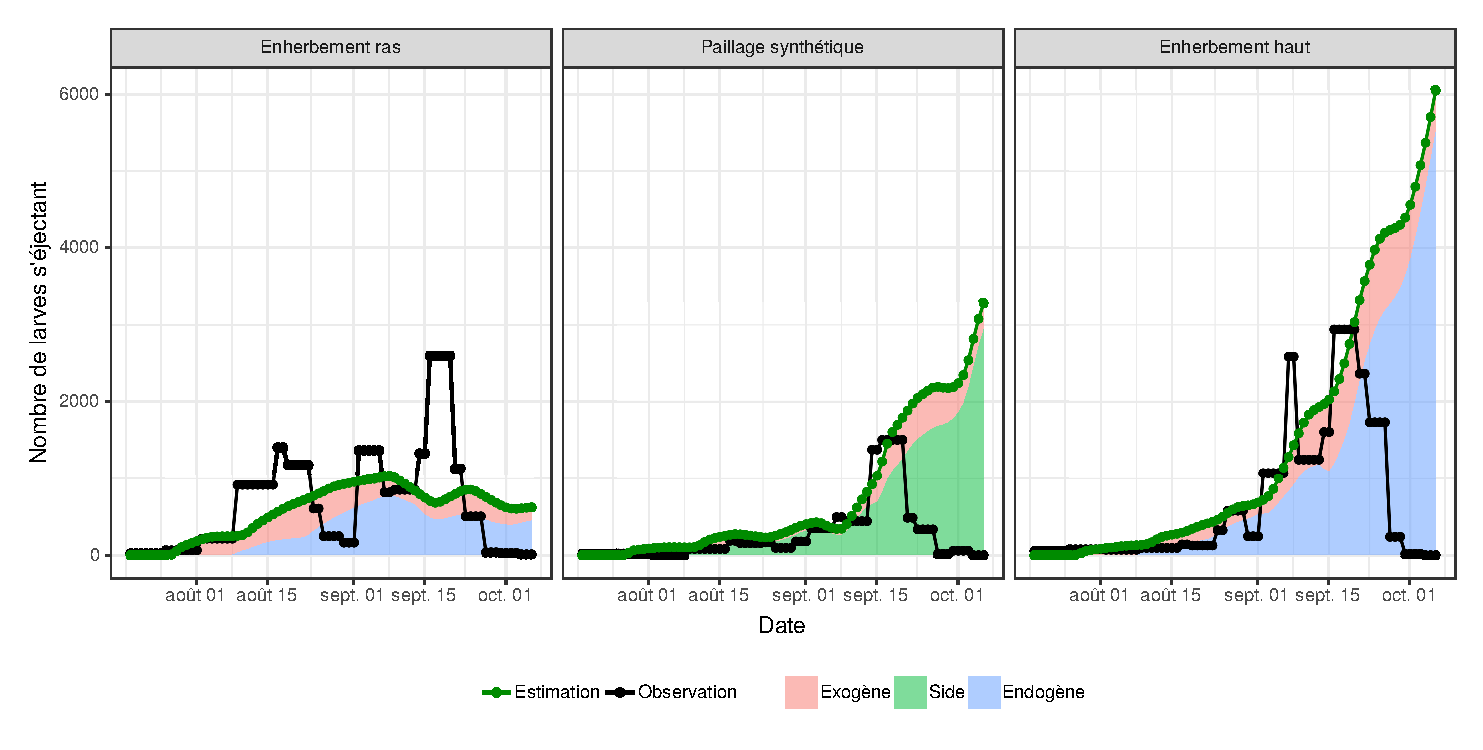
\epsfig{file = plots/max_erps.eps, scale = 0.65}
  
 \caption{Dynamiques estimées avec un jeu de paramètres vérifiant $\mu_{\text{ER}} < q_{0.1}\left( \mu_{\text{ER}} \right)$ et $\mu_{\text{EH}} > q_{0.9}\left( \mu_{\text{EH}} \right)$.}
 
 \label{fig:erps}
\end{figure}

\newpage
On peut essayer d'être bon sur tous les critères en minimisant la norme 1 (voir figure~\ref{fig:all}).

\begin{center}
\begin{tabular}{lllll}
$\gamma$ & $p_m$ & $\mu_{\text{ER}}$ & $\mu_{\text{EH}}$ & $k$\\
0.010 & 0.591 & 1.000 & 1.000 & 54.119
\end{tabular}
\end{center}


\begin{figure}[ht]
 \centering
 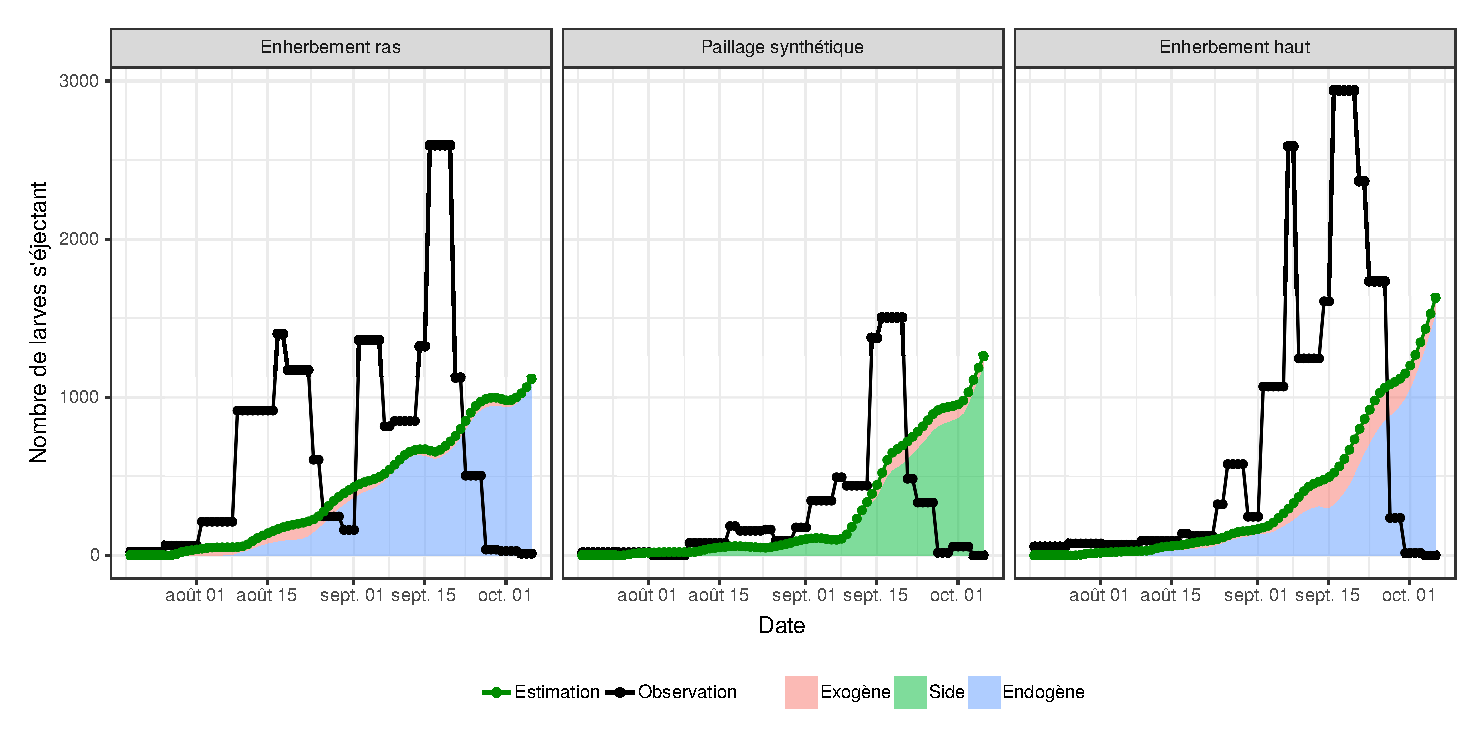
\epsfig{file = plots/all.eps, scale = 0.65}
  
 \caption{Dynamiques estimées avec un jeu de paramètres mimisant la norme 1 des quatre critères.}
 
 \label{fig:all}
\end{figure}


\section{Prochaines étapes}

--- Inclure la saisonnalité;

--- inclure le $\mu_{\text{global}}$ dans la calibration.


\clearpage
\bibliography{calib} 
\bibliographystyle{apalike}






\end{document}

